
%\section{Properties of the chords and variation of length}

In this section we obtain some  properties of chords of convex curves and their applications in billiard orbits.
 
Consider two regular convex curves $\gamma$ and $\Gamma$ parametrized by arc lengths $s$ and $t$. 
Let $l(s,t)=|\gamma(s)-\Gamma(t)|$, $\theta(s,t) $ the angle between $\gamma^\prime(s)$ and $V(s,t)=\Gamma(t)-\gamma(s)$ and  $\eta(s,t) $ the angle between $\Gamma^\prime(t)$ and $V(s,t)$. See Fig. \ref{fig:appC-1corda}.

Consider the Frenet frames $\{\gamma^\prime (s), N_\gamma\}$ and $\{\Gamma^\prime (t), N_\Gamma\}$ along $\gamma$ and $\Gamma$.  Denote the curvatures by $k_\gamma$ and 
$k_\Gamma$.

\begin{figure}[H]
	\begin{center}
	%	\def\svgwidth{0.75\textwidth}
	 %	\input{pics_tex/curva_convexa.eps_tex}
		 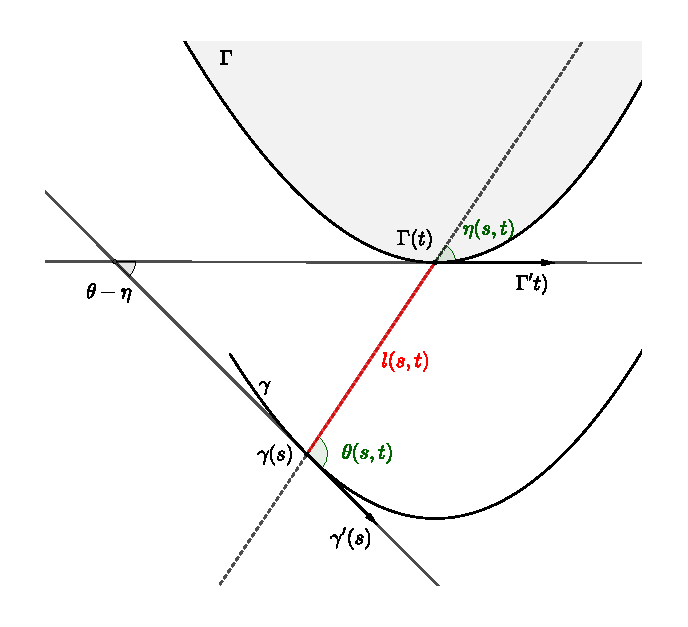
\includegraphics[scale=0.7]{ pics_appC_080_cordas_duas_curvas.pdf}
		\caption {Pair of curves and variations of length and angles.\label{fig:appC-1corda}}
	\end{center}
\end{figure}

\begin{proposition}  In the above conditions it follows that:


	\begin{equation}
\aligned
dl&= -\cos\theta\;   ds + \cos\eta\;   dt\\
d\theta &=\left( \frac{\sin\theta }{l }-k_{ \gamma}(s)\right) ds -\frac{\sin\eta}{l } dt\\
d\eta &=  \frac{\sin\theta }{l } ds  - \left(  \frac{\sin\eta}{l } + k_{\Gamma }(t)\right)  dt
\endaligned
\label{eqn:appC-variacaoL}
\end{equation}
\label{prop:appC-variacaoL}
\end{proposition}

\begin{proof} 
	We have that 
	\[  df=\frac{\partial f}{\partial s} ds +\frac{\partial f}{\partial t} dt\]
	
	From the equation \[ l^2= \langle \Gamma(t)-\gamma(s),\Gamma(t)-\gamma(s)\rangle \]
	it follows that
	\begin{align*}
	 2l \frac{\partial l}{ \partial s} &= -2\langle  \gamma^\prime(s), \Gamma(t)-\gamma(s)\rangle= -2l\cos\theta \;  \;    \Rightarrow\;  \;  l_s=-\cos\theta \\
	 %
	  2l \frac{\partial l}{ \partial t} &=  2\langle  \Gamma^\prime(t), \Gamma(t)-\gamma(s)\rangle=  2l\cos\eta \;  \;  \Rightarrow\;  \;   l_t=\cos \eta
	\end{align*}
	
	From the equations 
	\[  l(s,t)  \cos\theta =\langle  \gamma^\prime(s), \Gamma(t)-\gamma(s)\rangle,  \;\;   l(s,t)  \cos\eta   =\langle  \Gamma^\prime(t), \Gamma(t)-\gamma(s)\rangle   \]
	it follows that
	
		\begin{align*}
   l_s\cos\theta- l \theta_s\sin\theta   & =  \langle  \gamma^{\prime\prime}(s), \Gamma(t)-\gamma(s)\rangle- \langle  \gamma^\prime(s), \gamma^\prime(s)\rangle\\
	&  =  \langle \gamma^{\prime\prime}(s), l\cos \theta \gamma^\prime +l\sin\theta N_{\gamma}(s) \rangle-1\\
	 & =  l\sin\theta k_{\gamma}(s) -1\\
	 %
	  l_t\cos\theta- l \theta_t\sin\theta   & =  \langle  \gamma^{\prime }(s), \Gamma^\prime(t) \rangle =\cos( \theta-\eta)  = \cos( \eta-\theta) \\
%
	 l_s\cos\eta   -l \eta_s\sin\eta   & =  \langle  \gamma^{\prime }(s), \Gamma^\prime(t) \rangle =\cos( \theta-\eta)\\
	 %
	   l_t\cos\eta- l \eta_t\sin\eta  & =  \langle  \Gamma^{\prime\prime}(t), \Gamma(t)-\gamma(s)\rangle+ \langle  \Gamma^\prime(t), \Gamma^\prime(t)\rangle\\
	 & =  \langle \Gamma^{\prime\prime}(t), l\cos \eta \Gamma^\prime +l\sin\eta N_{ \Gamma} (t) \rangle+1 	\\
	  &  = \ k_{\Gamma}l \sin\eta +1 \\
%	 
	 	\end{align*}
	 	Performing the calculations leads to the result.   
\end{proof}

\begin{proposition}
	In the same conditions above but with arc length  parameters $s$ and $t$ it follows that
	\begin{equation}
	\aligned
	 l_{ss}&=  \sin\theta \left(\frac{\sin\theta}{l}-k_{\gamma}(s)\right)  \\
	 l_{st}&=  \frac {\sin\theta \sin\eta}{l}  \\
	 l_{tt}&=\sin\eta \left(\frac{\sin\eta}{l}-k_{\Gamma}(s)\right) 
		\endaligned
		\end{equation}
\end{proposition}

\begin{proof}
Follows directly from differentiation of  \cref{eqn:appC-variacaoL}.
\end{proof}

\begin{proposition}
	In the same conditions above but with arbitrary parameters $s$ and $t$ it follows that
	\begin{equation}
	\aligned
	dl &= -|\gamma'(s)|  \cos\theta  \; ds + |\Gamma^\prime(t)|  \cos\eta\;  dt\\
 	d\theta &=|\gamma'(s)|  \left( \frac{\sin\theta }{l }-k_\gamma(s) \right)ds     - \frac{ |\Gamma^\prime(t) | \sin\eta}{l }\;dt\\
 d\eta&=   \frac{ |\gamma'(s)| \sin\theta }{l } \;  ds  - |\Gamma^\prime(t)| \left(  \frac{\sin\eta}{l }+k_\Gamma(t) \right) \;  dt
\endaligned
\label{eq:appC-variacaoL2}
\end{equation}
\label{prop:appC-variacaoG}
\end{proposition}

\begin{proof}
Similar to the that given in \cref{prop:appC-variacaoL}.
\end{proof}

Consider a   closed smooth planar strictly convex curve $\gamma:[0,L]\to \mathbb {R}^2$. Let $P_0=[x_0,y_0]\in \mathbb{R}^2$ be a fixed point and draw the tangent lines to $\gamma$ at $\gamma(u_0)$ and $\gamma(v_0)$, passing through $P_0$ in the exterior region of $\gamma$.
Consider the set defined by:
\begin{align*}
F(P,u,v)&=|P-\gamma(u)|+|P-\gamma(v)|-L(\gamma(u),\gamma(v))=F(P_0,u_0,v_0)0)0\\
G(P,u)& =[P-\gamma(u),\gamma'(u)]=0,\; H(P,v)=[P-\gamma(v),\gamma'(v)]=0
\end{align*}
where $L(u,v)$ is the length of the chord $\gamma([u,v])$ (arc of the curve $\gamma_{|[u,v]}$ between $\gamma(u)$ and $\gamma(v)$).
See \cref{fig:appC-graves-convex}.
\begin{figure}
    \centering
    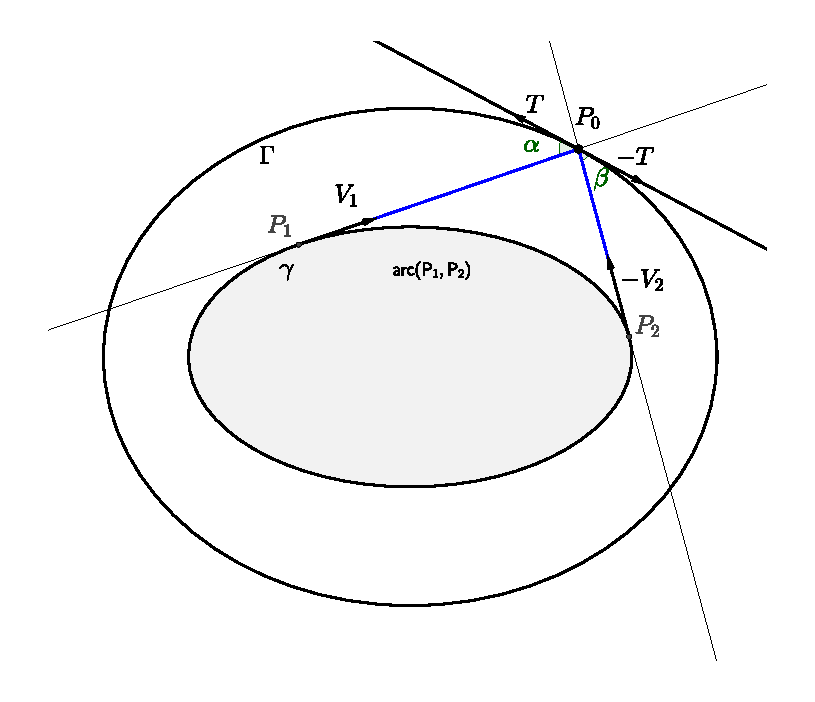
\includegraphics[scale=0.6]{zappC/pics/pics_appC_040_gravesgeral.pdf}
    \caption{String construction of the convex curve $\Gamma$. \label{fig:appC-graves-convex}}
   
\end{figure}

\begin{proposition} In the above conditions, the
 set defined by \[F(P,u,v)=F(P_0,u_0,v_0)>0, \;\;\; G(P,u)=\,H(P,v)=0\]
is a regular curve and their  projection in the plane is a regular curve $\Gamma$ making equal angle with the two  tangent lines to $\gamma$.
 \label{prop:appC-Gamma}
\end{proposition}

\begin{proof}
Suppose that $\gamma$ is parametrized in graphic
form $(x,f(x))$. Let $l_1=\sqrt{1+f'(u)^2}$ and
$l_2=\sqrt{1+f'(v)^2}$.
The tangent lines to $\gamma$ at $x=u$ and $x=v$
are given by
\[ G(x,y,u)=y-f(u)-f'(u)(x-u)=0,\;\;\; H(x,y,v)=y-f(v)-f'(v)(x-v)\]

Let $P=(X,Y)$ be  point in the exterior region bounded by $\gamma$. We can suppose that $u<X<v.$
Therefore, 
\[F(P,u,v)=l_1(X-u)-l_2(X-v)-\int_u^v \sqrt{1+f'(x)^2}dx \]

Supposing, for the moment,  that $F=G=H=0$ defines  a regular curve.  Differentiating the equations $F=0$, $G=0$ and $H$ with respect to $X$ it follows that:

\begin{align*}
(1-\frac{du}{dX})l_1 &+(X-u)\frac{f'(u)f''(u)}{l_1}\frac{du}{dX}-(1-\frac{dv}{dX})l_2\\
    &-(X-v)\frac{f'(v)f''(v)}{l_2}\frac{dv}{dX}-l_2\frac{dv}{dX}+l_1\frac{du}{dX}=0
    \frac{dY}{dX}-f'(u)&=f''(u)(X-u)\frac{du}{dX}\\
    \frac{dY}{dX}-f'(v)&=f''(v)(X-v)\frac{dv}{dX}
\end{align*}
Eliminating $du/dX$ and $dv/dX$ from the above equations   it follows that
\[\frac{dY}{dX}=\frac{l_1-l_2}{l_2f'(u)-l_1f'(v)}\]
Consider the vectors

\[V_1=[1,f'(u)],\;\; V_2=[1,f'(v)],\;\; 
T=[l_2f'(u)-l_1f'(v),l_1-l_2]\]
We have that
$\cos\alpha=\frac{\langle V_1,T\rangle}{l_1|T|}=\frac{\langle - V_2,- T\rangle}{l_2|T|}=\cos\beta$. Finally we observe that for a convex curve we have that $T\ne 0$ for all $u\ne v.$ In fact, $T=0$ only if   $l_1=l_2$ and $f'(u)=f'(v)$. This  leads to parallel lines; a contradiction. This ends the proof.
\end{proof}

\begin{remark}
The above proof   was adapted from \cite{miller-1925}.
\end{remark}

\begin{remark}
The tangent vector $(v_1,v_2,v_2,v_4)$ to the curve defined implicitly in  \cref{prop:appC-Gamma} is given by:
{\small  
\begin{align*}
v_1&={\frac {l_1
^{2} l_2^{2} k \left( u \right) k \left( v \right)  \left( (u-v){f'(u)} +\Delta f \right)  \left( (u-v){f'(v)} +\Delta f \right)  \left( {f'(u)}\,{l_2}-{f'(v)}\,  
l_1 \right) }{ \left( {f'(v)}-{f'(u)} \right) ^{2}}}
\\
v_2&={\frac {l_1
^{2} l_2^{2} k \left( u \right) k \left( v \right)   \left( (u-v){f'(u)} +\Delta f \right)  \left( (u-v){f'(v)}  +\Delta f \right)  \left( {l_1}-{l_2} \right) }{
 \left(  {f'(v)}-{f'(u)} \right) ^{2}}}\\
v_3&={\frac { \left( (u-v){f'(u)} +\Delta f \right)  \left( {l_1
}\,{f'(u)}\,{f'(v)}+l_1^{2}{l_2}+{l_1}-2\,{l_2}
 \right) k(v) l_2^{2}}{{l_1}\, \left( {f'(u)}-{f'(v)
} \right) }}\\
v_4&=\frac{(f'(u) f'(v) l_2 + l_1 l_2^2 - 2 l_1 + l_2) ((u-v)f'(v)   + \Delta f) k(u) l_1^2 }{ ((f'(v) - f'(u)) l_2)}\\
 \Delta f& =f(v)-f(u)
\end{align*}
}
\end{remark}

 Let $\gamma$ be a convex curve of length $L=l(\gamma)>0$.
   For $P$  outside $\gamma$ let $ L(P)$   the length of a string through $P$ stretched tightly around $\gamma$. For each $r>L$, let $C_r=\{p\in\mathbb{R}^2: L(p)=r\}.$ Then  $C_r$ is the  boundary of a convex body $\Gamma$ having $\gamma$ as a caustic.
   
   
\begin{corollary}
  Any smooth closed strictly convex curve is a caustic of a convex billiard.
  \label{cor:appC-caustica}
\end{corollary}

\begin{proof}
 Let $\gamma$ be a convex curve of length $L=l(\gamma)>0$.
For $P$  outside $\gamma$ let $ L(P)$   the length of a string through $P$ stretched tightly around $\gamma$. For each $r>L$, let $C_r=\{p\in\mathbb{R}^2: L(p)=r\}.$ Then  $C_r$ is the  boundary of a convex body $\Gamma$. By Proposition \cref{prop:appC-Gamma},   $\gamma$ is a caustic of $C(r)$.
\end{proof}
  
   \begin{proposition} Consider a billiard in a region with boundary a convex curve $\Gamma$. Let $\gamma$ be the caustic of a family of orbits as shown in Fig. \ref{fig:appC-corda2}. Then for any $x\in \Gamma$
   \[ |x-y|+|x-z|-arc(y,z) =\text{cte}.\]
   Here $y,z\in \gamma$ are the points of tangency of the billiard orbit passing through $x$ with the caustic and $arc(x,z)$ is the length of caustic between $y$ and $z$.
    \begin{figure}[H]
	\begin{center}
	%	\def\svgwidth{0.55\textwidth}
	%	\input{pics_tex/corda2.eps_tex}
		 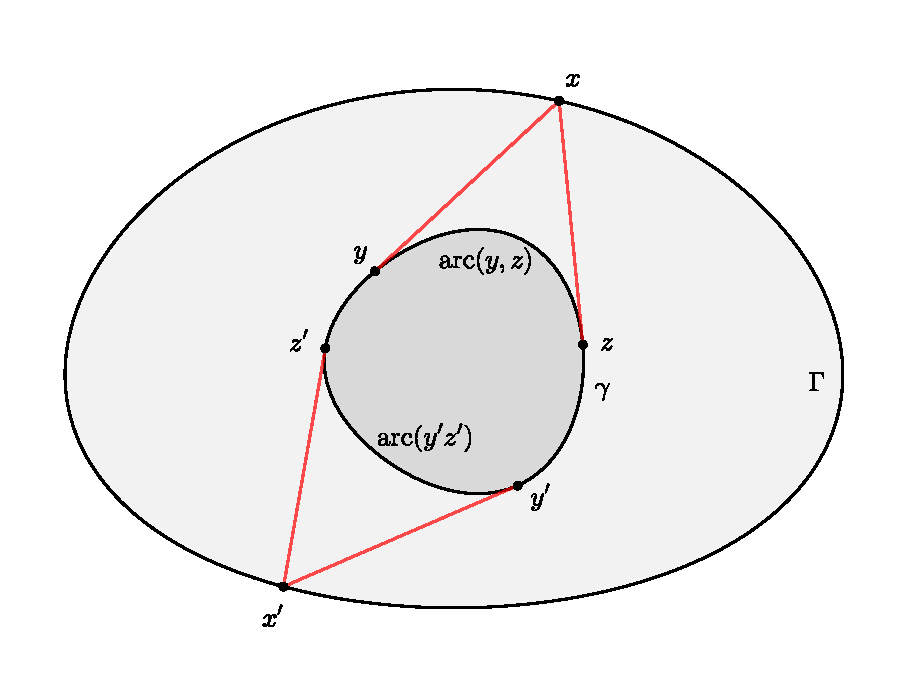
\includegraphics[scale=0.6]{zappC/pics/pics_appC_100_duas_curvas.pdf}
		\caption { Tangents to a caustic and length of chords.\label{fig:appC-corda2}}
	\end{center}
\end{figure}
   \end{proposition}
   
   \begin{proof} [Sketch of Proof.] Let  $\Gamma(t)$  be a  parametrization of the boundary. Consider also local parametrizations   $\gamma_1(t)$ and $\gamma_2(t)$ of the caustic $\gamma$  with $\gamma_1(0)=z$, $\gamma_2(0)=y$, and $\Gamma(0)=x$. Suppose that all curves are   counterclockwise oriented.
   Let also the caustic parametrized by natural parameter $s$. Then
   \[\gamma(s)=\gamma_1(t)=\Gamma(t)+\lambda(t) d_1(t), \;\;\gamma(s)=\gamma_2(t)=\Gamma(t)+\lambda(t) d_21(t).\]
   Here $d_1$ and $d_2$ are the directions of the tangent lines $xy$ and $xz$ to the caustic.
   
   Let $l_1(t)= |\Gamma(t)-\gamma_1(t)|$ with $l_1(0)=|x-z|$. Also define $l_2(t)= |\Gamma(t)-\gamma_2(t)|$ with $l_2(0)=|x-y|$.
   
   By Proposition \ref{prop:appC-variacaoG} it follows that
   \begin{align*}
   dl_1 &=\cos\eta |\Gamma^\prime(t)|dt-|\gamma_1^\prime(s)|ds\\
    dl_2 &=|\gamma_2^\prime(s)|ds-\cos\eta |\Gamma^\prime(t)|dt
   \end{align*}
   Here we used   the condition of billiard orbit at the point $x$ (angle of incidence is equal to angle of reflection) and that $\cos\theta_{1,2}=\pm 1$ (caustic is tangent to billiard orbits, taking into account     the orientation).
   Therefore it follows that
   \[d(l_1+l_2)-|\gamma_2^\prime(s)|ds+|\gamma_1^\prime(s)|ds=0.\]
   Integrating it follows that
   \[l_1(a)-l_1(0)+l_2(a)-l_2(0)=arc(\gamma_1(0),\gamma_1(a))-arc(\gamma_2(0),\gamma_2(a))\]
   Therefore,
   \[l_1(a)+l_2(a)-arc(\gamma_1(a),\gamma_2(a))=l_1(0)+l_2(0)-arc(\gamma_1(0),\gamma_2(0)).\]
   
   
   \end{proof}